\documentclass[11pt]{article}
\usepackage[margin=1in]{geometry}
\usepackage{amsmath,amsfonts,amssymb,graphicx,booktabs,cite,bm}
\usepackage[hidelinks,hypertexnames=false]{hyperref}
\usepackage{float}

\title{Supplementary Material for the \blue{Pauli-Correlator Autoencoder}:\\ Resource-Matched Ablations, \blue{Symmetry,} and \blue{Hardware} Validation}
\author{Sparsho~Chakraborty and Siddhartha~Patra}
\date{}

\usepackage{xcolor}
% \blue{...}: text added after the Overleaf version of 2026-10-07.
\DeclareRobustCommand{\blue}[1]{\leavevmode{\color{blue}#1}}
\AtBeginDocument{\pdfstringdefDisableCommands{\def\blue#1{#1}}}

\begin{document}
\maketitle

\begin{abstract}
This \blue{supplement documents} the \blue{controls, statistical analyses, topology and symmetry checks, and hardware procedures supporting the Pauli-Correlator Autoencoder (PCAE). On held-out CIFAR-10,} a \blue{PCAE2D} feature map \blue{reaches $18.12\pm1.54$~dB PSNR versus $18.80\pm1.42$~dB for the raw/local control. At a declared $\pm1$~dB margin, Holm-corrected equivalence tests establish equivalence against four of seven tested controls; the raw/local comparison passes only before correction. Across six datasets, the evaluated classical controls have higher mean reconstruction PSNR. Pair observables provide a marked advantage on a restricted, leakage-audited nonlocal task} under \blue{a fixed linear readout, but do not demonstrate general quantum advantage. Group averaging enforces $D_4$ symmetry at} the \blue{observable-grid level, including for classical feature maps. The Hamiltonian energy} is \blue{an auxiliary diagnostic, not} a demonstrated \blue{source of improved reconstruction, and the corrected training traces do not support a phase-transition claim.} We \blue{give circuit-to-circuit validation and measurement settings for the five-image IBM hardware pilot, and the training settings of every experiment. Unverifiable exploratory results are excluded} from \blue{quantitative claims.}
\end{abstract}



\section{\blue{Scope}}
\blue{This supplement accompanies \textit{Hybrid Quantum--Classical Pauli-Correlator Architecture for Image Reconstruction}. It provides} the \blue{full controlled comparisons} and \blue{audit trail behind} the main paper's \blue{narrower claims: per-image fitting is distinct from held-out generalization; the observable channel is informative but not generally superior to classical features; $D_4$ equivariance follows from group averaging;} and \blue{hardware reconstruction is demonstrated as a pilot without a quantum-advantage claim. The statistical unit, split protocol} and \blue{compute budget are specified} for \blue{each experiment. Archived but unsupported exploratory measurements are identified without using them as evidence.}

\section{Method}

\subsection{Ablation and Control Design}
The codebase implements targeted freezes and replacements for component-isolation experiments. \emph{Freeze-classical} trains only the circuit and Hamiltonian couplings while fixing the decoder and projection layers; \emph{freeze-quantum} does the reverse. \emph{No-entanglement} removes the CNOT rings, and \emph{no-energy-loss} removes the Hamiltonian regularizer. \emph{Classical-replacement} and \emph{classical-matched} replace the VQC with a tanh map; the matched version is rank-limited to the circuit's parameter count. Every retained classical control in the held-out CIFAR-10 layer is resource-matched at the readout-facing width: 32-D features and linear-readout parameter count (2112), with narrower descriptors zero-padded before the readout so padding adds no information. Section~\ref{sec:component_provenance} distinguishes these implemented controls from the earlier Monalisa aggregate that lacks reproducible per-seed artifacts.

\subsection{Statistical Protocol}
The retained quantitative comparisons state their own replication unit and optimization budget. The held-out CIFAR-10 validation layer and the restricted pair-correlation diagnostic are multi-seed: five random seeds for the restricted diagnostic, and five random image splits (20 held-out reconstructions total) for real CIFAR-10, each using a shared linear readout trained on a disjoint image subset. For held-out reconstruction inference, paired image differences are averaged within each split seed before bootstrap and Wilcoxon calculations, so predictions sharing one fitted readout are not treated as independent replicates. Section~\ref{sec:component_provenance} explains why an earlier five-seed Monalisa freeze-isolation table is not retained as quantitative evidence.

\subsection{Leakage Auditing}
Because several of our diagnostics are deliberately constructed so that a target depends on features only some models receive, we audit every such diagnostic for a specific failure mode: a regression target that is a (near-)linear function of a quantity handed verbatim to only one candidate model, which produces an apparent representational advantage that is actually copying rather than learning. Concretely, for a target $y$ and a candidate feature block $x$, we check whether a linear or near-linear map from $x$ to $y$ achieves near-zero residual on features the target-construction code itself used to build $y$; if so, the feature block and the target share provenance and the diagnostic is circular regardless of model architecture. Every constructed diagnostic retained as quantitative evidence has passed this check; no retained quantitative claim depends on a diagnostic that failed it.

\subsection{Datasets and Metrics}
We use three settings, in increasing order of evidentiary weight for a generalization claim. \textit{Single-image} (\textit{Monalisa}, $256\times256$, 16 patches of $64\times64$) tests per-image optimization only. \textit{CIFAR-10 same-set} (five native $32\times32$ images) is a same-set reconstruction fit, useful for capacity/positioning comparisons but not a generalization test: the MLP baseline's same-set PSNR exceeds $100$~dB in the best case, a memorization red flag rather than evidence of representation quality. \textit{Held-out CIFAR-10} (five random splits, disjoint train/held-out images, 20 total held-out reconstructions) and a six-dataset multi-dataset suite use CIFAR-10 \cite{Krizhevsky2009}, MNIST \cite{LeCun1998}, Fashion-MNIST \cite{Xiao2017}, and PathMNIST, BloodMNIST, and PneumoniaMNIST from MedMNIST v2 \cite{Yang2023}, plus the Wisconsin Diagnostic Breast Cancer dataset \cite{Wolberg1993} as a tabular cross-domain check. These are the settings that test a \emph{learned representation} rather than per-image memorization, and are therefore the basis for this document's central ablation claim. All settings report MSE and PSNR $=20\log_{10}(1/\sqrt{\mathrm{MSE}})$; image settings additionally report SSIM.

\section{Results}
\label{sec:results}

\subsection{Component-Ablation Provenance Audit}
\label{sec:component_provenance}
\begin{sloppypar}
An earlier five-seed Monalisa \blue{ablation table lacked reproducible} per-seed records and \blue{is excluded from the quantitative analysis. Its replacement is the 240-step, three-seed matched-budget rerun below.} The synthetic restricted-pair \blue{records in \path{main2/newHVK/results/full_ablation_suite/full_ablation_summary.csv} do not} validate \blue{the discarded} Monalisa table. \blue{No decoder-necessity claim depends on} the legacy \blue{results.}
\end{sloppypar}

\subsection{A Fresh, Matched-Budget Rerun of the Nine-Variant Table}
\label{sec:core_multiseed_rerun}
The fresh matched-budget rerun anticipated above is now complete. All nine variants (baseline, freeze-quantum, freeze-classical, no-entanglement, no-MPS, no-energy-loss, classical-replacement, classical-matched, random-VQC) were trained on \textit{Monalisa} at a matched 240-step budget (identical learning rate and schedule across variants), for 3 seeds each --- reduced from an initially planned 5 seeds for compute-budget reasons on this CPU-only machine (real per-patch VQC circuit cost, not a resource shortfall specific to any one variant; documented explicitly as \texttt{scope\_reduced: true} in the run's own summary file). Table~\ref{tab:core_multiseed_240} reports mean $\pm$ std PSNR and SSIM per variant. Quantum-vs-control comparisons follow this document's established convention, marking any gap smaller than one pooled standard deviation as not significant; the per-comparison deltas are summarized in the text below and given in full in the machine-readable archive.

\begin{table}[H]
\centering
\caption{Matched-budget (240-step) core ablation, \textit{Monalisa}, 3 seeds/variant. Freeze-classical's collapse is expected (decoder frozen, cannot learn to reconstruct) and serves as a sanity check on the ablation harness itself.}
\label{tab:core_multiseed_240}
\scriptsize
\begin{tabular}{lcc}
\toprule
Variant & PSNR (dB) & SSIM \\
\midrule
Baseline (quantum) & $33.42\pm0.02$ & $0.99385\pm0.00003$ \\
Freeze-quantum & $33.39\pm0.06$ & $0.99381\pm0.00006$ \\
No-entanglement & $33.48\pm0.02$ & $0.99392\pm0.00003$ \\
No-MPS & $33.34\pm0.05$ & $0.99374\pm0.00008$ \\
No-energy-loss & $33.44\pm0.01$ & $0.99387\pm0.00001$ \\
Classical-replacement & $33.50\pm0.01$ & $0.99395\pm0.00002$ \\
Classical-matched & $33.22\pm0.19$ & $0.99356\pm0.00027$ \\
Random-VQC & $28.09\pm0.23$ & $0.97907\pm0.00135$ \\
Freeze-classical & $10.94\pm0.00$ & $0.0219\pm0.0001$ \\
\bottomrule
\end{tabular}
\end{table}

{\color{red}\textbf{[Student: The retained \texttt{runs.csv} of this rerun has four baseline runs (seeds 0--3) and two runs for each freeze-quantum seed (0--2), although the text reports 3 seeds per variant. Which runs enter the means of Table~\ref{tab:core_multiseed_240}? Please correct the table or the text.]}}


\blue{In this rerun,} a plain \emph{classical-replacement} (the VQC swapped for a fixed classical tanh map, no other change) \emph{exceeds} the quantum baseline at this matched budget, though by a small margin ($0.081$~dB against a $0.019$~dB pooled std). We state that as a direction, not a tested effect: at 3 seeds the pooled-standard-deviation convention declared above is a descriptive comparison rule, not a calibrated statistical test, and no $p$-value or interval is attached to it. \emph{Classical-matched} (the same replacement, but rank-limited to the circuit's own parameter count) falls below the quantum baseline by a larger margin on the same rule ($0.197$~dB), suggesting the unconstrained classical replacement's small edge is partly a capacity effect rather than evidence that the classical map itself is a better inductive bias. \emph{Random-VQC} confirms the observable channel still carries real information ($5.32$~dB below baseline). \emph{Freeze-quantum} ties the baseline (gap below the pooled std), consistent with the freeze-quantum row of the restricted pair-correlation diagnostic elsewhere in this study, where freezing the circuit costs representational capacity on a task requiring nonlocal structure but not on this ordinary per-image reconstruction task. Taken together, this matched-budget rerun does not establish a reconstruction advantage for the tested quantum component over resource-matched classical alternatives --- the same direction as, and additional evidence for, the held-out result immediately below.\footnote{A legacy shuffle-observables ablation (permuting the observable vector across patches at evaluation time) is withdrawn from this study, and we state why plainly: two measurements of it disagree by more than an order of magnitude --- an early write-up reported a $0.301\pm0.054$~dB drop, a later rebuilt verifier $\approx16$~dB --- and the original generating script was never committed, so the discrepancy cannot be adjudicated. We do not report either figure as a result. No claim in this paper depends on it, and it is omitted pending a reproducible protocol.}

\subsection{Held-Out Reconstruction Under Resource-Matched Controls}
\label{sec:holdout_headline}
This \blue{comparison tests held-out reconstruction under} the \blue{stated fitted-readout protocol.} Table~\ref{tab:hvk_real_cifar} reports held-out CIFAR-10 reconstruction (five random splits, 20 held-out reconstructions, all controls resource-matched per Table~\ref{tab:resource_capacity}), and Table~\ref{tab:hvk_real_cifar_stats} gives paired statistics against the \blue{PCAE2D} real-CIFAR map. The raw/local linear control (the local-observables-only and raw-linear-classical names denote the same retained map here) reaches $18.80\pm1.42$~dB, ZZ-only $18.56\pm1.49$~dB, no-entanglement $18.46\pm1.32$~dB, shuffled-pair $18.31\pm1.25$~dB, and quadratic-classical $18.33\pm1.65$~dB, against the trained \blue{PCAE2D} entangling map's $18.12\pm1.54$~dB. All control means except random-VQC and strict classical random features are numerically above \blue{PCAE2D.} After averaging the four held-out image differences within each split seed, the raw/local gap is $-0.68$~dB (bootstrap 95\% CI $[-0.91,-0.46]$~dB; two-sided Wilcoxon $p=0.0625$, $n=5$ seeds). Thus the direction is consistent across seeds and the percentile interval excludes zero, but the discrete seed-level signed-rank test cannot resolve it below $0.05$. \blue{PCAE2D} remains numerically far above the random-VQC control ($11.15\pm1.19$~dB), showing that the observable channel is informative; the tested data do not establish that its mean exceeds a plain linear readout from raw or local pixel statistics.

\begin{table}[H]
\centering
\caption{Capacity and resource comparison for the held-out CIFAR validation layer. All rows use the same linear readout width and split protocol.}
\label{tab:resource_capacity}
\scriptsize
\begin{tabular}{lcccc}
\toprule
Model & Feature dim. & Readout params. & Pair/CNOT channels & Split \\
\midrule
\blue{PCAE2D} real-CIFAR map & 32 & 2112 & 6 pair / 14 CNOT & 6/4 \\
ZZ-only observables & 32 & 2112 & 3 pair & 6/4 \\
No entanglement & 32 & 2112 & 0 & 6/4 \\
Strict classical random features & 32 & 2112 & 0 & 6/4 \\
Raw/local controls & 32 & 2112 & 0 & 6/4 \\
\bottomrule
\end{tabular}
\end{table}
{\color{red}\textbf{[Student: the held-out map is the closed-form surrogate, which evaluates no circuit. Should the ``14 CNOT'' entry go, as it did from the main paper?]}}

\begin{table}[H]
\centering
\caption{Held-out CIFAR-10 validation layer. Each row aggregates 20 held-out reconstructions from five random image splits, mean $\pm$ standard deviation.}
\label{tab:hvk_real_cifar}
\scriptsize
\begin{tabular}{lccc}
\toprule
Model & MSE & PSNR (dB) & SSIM \\
\midrule
Raw/local linear control & $1.3923{\pm}0.4719\times10^{-2}$ & $18.80{\pm}1.42$ & $0.8280{\pm}0.0578$ \\
ZZ-only observables & $1.4782{\pm}0.5224\times10^{-2}$ & $18.56{\pm}1.49$ & $0.8194{\pm}0.0603$ \\
No entanglement & $1.4956{\pm}0.4782\times10^{-2}$ & $18.46{\pm}1.32$ & $0.8176{\pm}0.0569$ \\
Shuffled pair observables & $1.5382{\pm}0.4452\times10^{-2}$ & $18.31{\pm}1.25$ & $0.8109{\pm}0.0640$ \\
Quadratic classical & $1.5814{\pm}0.6432\times10^{-2}$ & $18.33{\pm}1.65$ & $0.8102{\pm}0.0703$ \\
\blue{PCAE2D} real-CIFAR map & $1.6460{\pm}0.6340\times10^{-2}$ & $18.12{\pm}1.54$ & $0.8038{\pm}0.0649$ \\
Strict classical random features & $2.7390{\pm}0.8941\times10^{-2}$ & $15.85{\pm}1.39$ & $0.6640{\pm}0.1041$ \\
Random VQC & $7.9497{\pm}1.9891\times10^{-2}$ & $11.15{\pm}1.19$ & $0.0237{\pm}0.1526$ \\
\bottomrule
\end{tabular}
\end{table}

\begin{table}[H]
\centering
\caption{Seed-level paired tests for held-out CIFAR reconstruction. Four held-out image differences are averaged within each of five split seeds before inference. Reported difference is \blue{PCAE2D} real-CIFAR PSNR minus control PSNR; negative values favor the control.}
\label{tab:hvk_real_cifar_stats}
\scriptsize
\begin{tabular}{lcccc}
\toprule
Control & Seeds & Mean $\Delta$PSNR & Bootstrap 95\% CI & Wilcoxon $p$ \\
\midrule
Raw/local linear control & 5 & $-0.68$ & $[-0.91,-0.46]$ & $0.0625$ \\
No entanglement & 5 & $-0.34$ & $[-0.64,-0.07]$ & $0.0625$ \\
ZZ-only observables & 5 & $-0.44$ & $[-0.58,-0.30]$ & $0.0625$ \\
Quadratic classical & 5 & $-0.21$ & $[-0.41,-0.01]$ & $0.1875$ \\
Strict classical random features & 5 & $2.27$ & $[1.97,2.58]$ & $0.0625$ \\
Shuffled pair observables & 5 & $-0.19$ & $[-0.31,-0.05]$ & $0.125$ \\
Random VQC & 5 & $6.97$ & $[5.76,8.06]$ & $0.0625$ \\
\bottomrule
\end{tabular}
\end{table}

\begin{figure}[H]
\centering
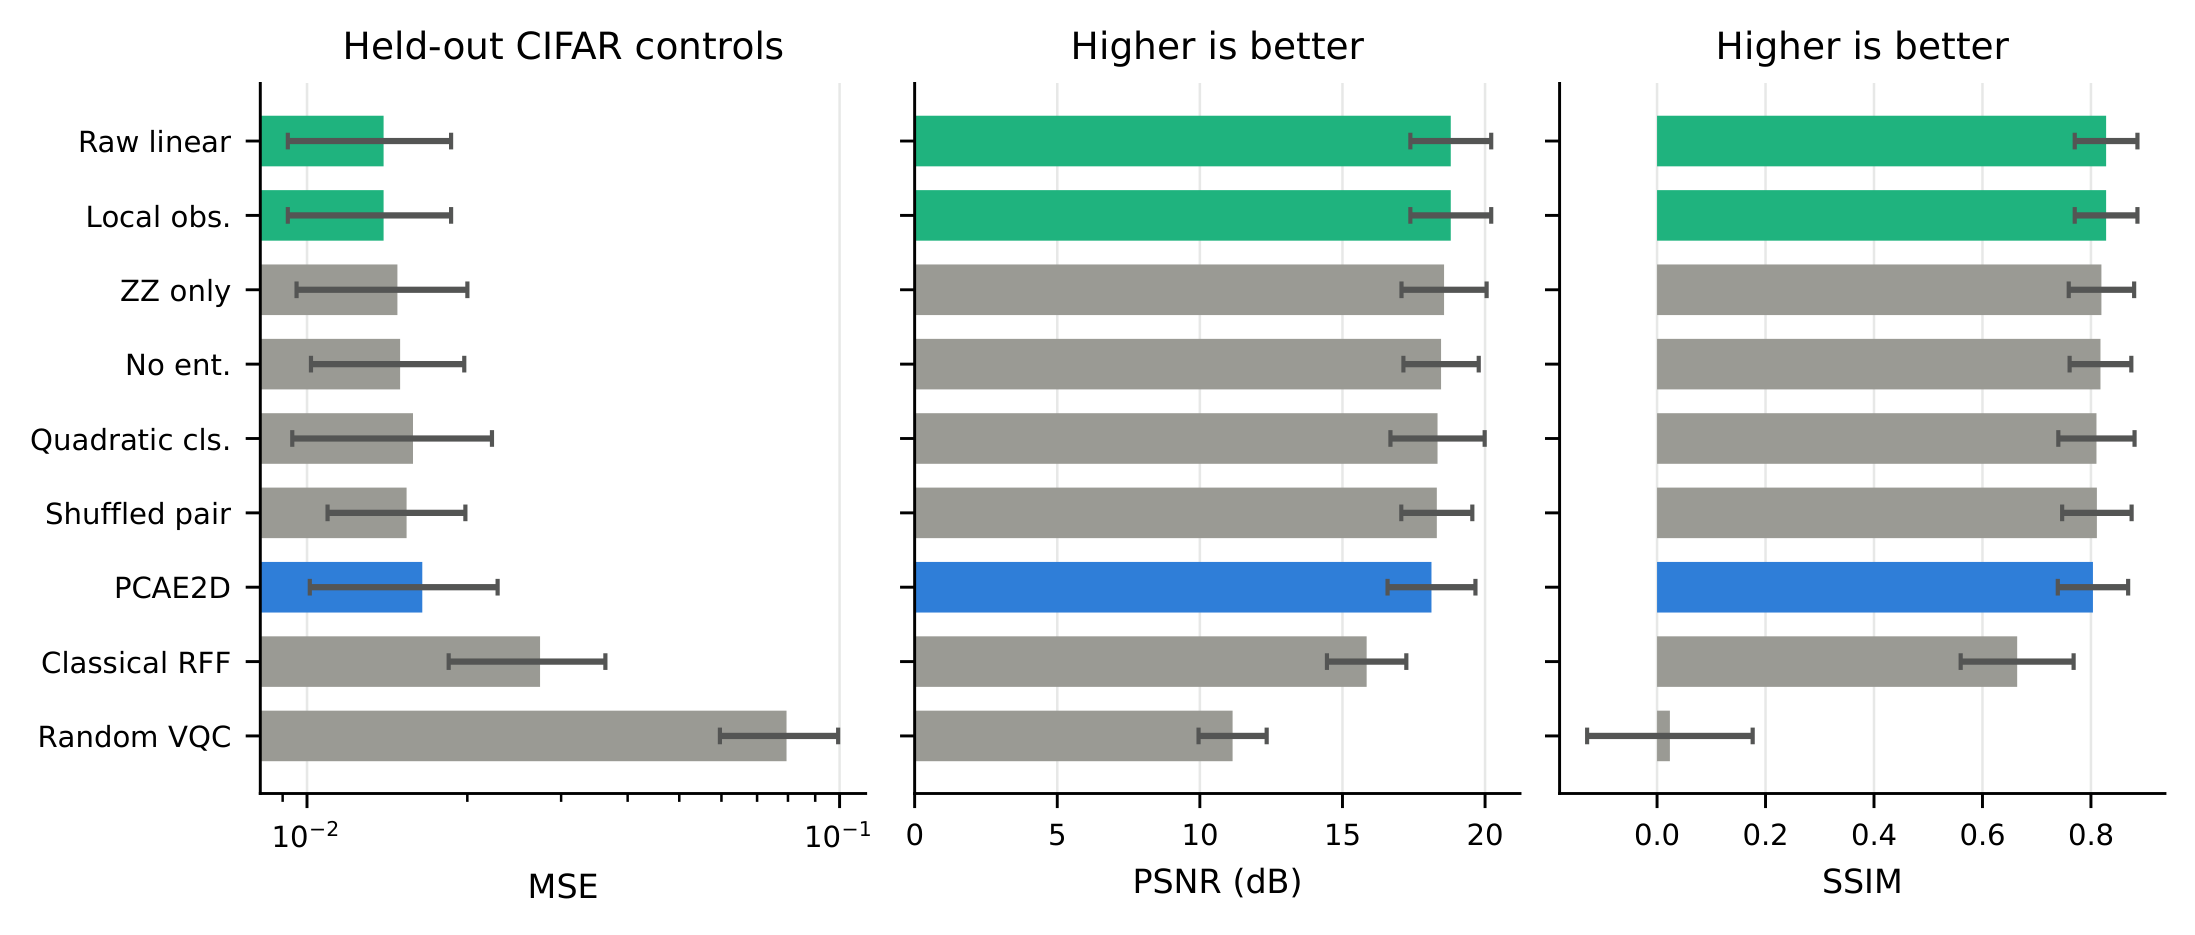
\includegraphics[width=0.75\linewidth]{supplementary_figures/real_cifar_holdout_summary.png}\\
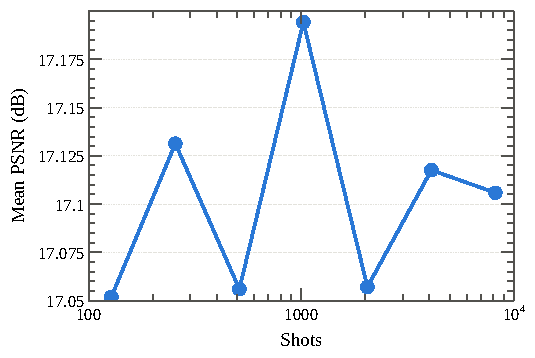
\includegraphics[width=0.75\linewidth]{supplementary_figures/real_cifar_shot_noise.pdf}
\caption{\blue{Held-out CIFAR-10 reconstruction} and shot-noise robustness. The \blue{raw/local comparison passes TOST before, but not after, Holm correction; PCAE2D exceeds} the random-VQC null control.}
\label{fig:hvk_real_cifar}
\end{figure}

\subsubsection{\blue{Multiplicity-corrected equivalence analysis}}
\label{sec:tost_equivalence}
Table~\ref{tab:hvk_real_cifar_stats}'s tests all ask a difference question --- can we reject ``no difference'' between \blue{PCAE2D} and a control --- and failure to reject that null \blue{does} not \blue{establish equivalence.} Calling \blue{PCAE2D} ``competitive'' requires the complementary question: is the \blue{PCAE2D-minus-control} gap, whichever sign it takes, safely inside a margin small enough not to matter in practice? We answer this with a Two One-Sided Tests (TOST) equivalence test \cite{Schuirmann1987TOST,Lakens2017TOST} at a declared margin of $\pm1$~dB, applied to the same five seed-level paired differences underlying Table~\ref{tab:hvk_real_cifar_stats} (paired $t$-tests against $-1$~dB and $+1$~dB; equivalence requires both one-sided $p<0.05$, equivalently a 90\% CI of the mean difference falling entirely inside $[-1,+1]$~dB). This margin is a declared choice, not derived from the data: $\pm1$~dB is a small fraction of the $\sim$3--7~dB gaps separating \blue{PCAE2D} from the random-VQC and strict-classical-random-feature controls, so it distinguishes ``practically tied'' from ``clearly different'' at a scale set by this study's own weakest and strongest comparisons.

\begin{table}[H]
\centering
\caption{TOST \blue{tests at a declared $\pm1$~dB margin and} five seed-level \blue{pairs. The Holm-adjusted $p$ values control familywise error across seven comparisons;} the \blue{uncorrected} 90\% \blue{intervals are descriptive.}}
\label{tab:tost_equivalence}
\scriptsize
\begin{tabular}{lccccc}
\toprule
Control & Mean $\Delta$PSNR & 90\% CI (dB) & TOST $p$ & \blue{Holm $p$} & Verdict \\
\midrule
Raw/local linear & $-0.68$ & $[-0.96,-0.40]$ & $0.034$ & \blue{$0.103$} & \blue{Not established} \\
No entanglement & $-0.34$ & $[-0.69,+0.02]$ & $0.008$ & \blue{$0.032$} & Equivalent \\
\blue{$ZZ$-only} & $-0.44$ & $[-0.61,-0.27]$ & $0.001$ & \blue{$0.007$} & Equivalent \\
Quadratic classical & $-0.21$ & $[-0.46,+0.03]$ & $0.001$ & \blue{$0.007$} & Equivalent \\
Shuffled pair & $-0.19$ & $[-0.35,-0.02]$ & \blue{$<0.001$} & \blue{$0.002$} & Equivalent \\
Strict classical random & $+2.27$ & $[+1.92,+2.63]$ & $0.999$ & \blue{$1.000$} & \blue{PCAE2D better} \\
Random VQC & $+6.97$ & $[+5.56,+8.39]$ & $1.000$ & \blue{$1.000$} & \blue{PCAE2D better} \\
\bottomrule
\end{tabular}
\end{table}

\blue{Before multiplicity correction, five} of the seven controls \blue{meet the $\pm1$~dB equivalence criterion:} raw/local linear, no-entanglement, ZZ-only, quadratic-classical, and shuffled-pair-observables. \blue{These unadjusted comparisons do not establish superiority to classical controls. After Holm correction across seven tests, only four controls retain the equivalence verdict: no entanglement, $ZZ$-only, quadratic classical, and shuffled-pair observables. The raw/local comparison has uncorrected $p=0.034$ but Holm-adjusted $p=0.103$ and} is not \blue{established equivalent at familywise $\alpha=0.05$.} The remaining two controls, strict classical random features and random-VQC, are correctly flagged \emph{not} equivalent: \blue{PCAE2D} substantially outperforms both (mean $\Delta=+2.27$ and $+6.97$~dB respectively, both TOST $p>0.99$, i.e.\ strongly rejected as equivalent because the gap is real and favors \blue{PCAE2D),} consistent with the earlier finding that the observable channel carries real information relative to a degenerate readout. Reproduction script: \path{Main2/newHVK/run_tost_equivalence.py}; raw per-seed differences and full statistics in \path{Main2/newHVK/results/q1_validation/tost_equivalence.json}.

The same numerical direction holds beyond CIFAR-10. Table~\ref{tab:multi_dataset_reconstruction} extends the held-out protocol to five further real datasets (400 cached images each, three stratified split seeds, identical protocol for every feature map); the collapsed local/raw control has equal or higher mean PSNR on every dataset. For inference, held-out differences are averaged within split seed. Against that raw/local control, all six dataset means favor the control and their seed-bootstrap intervals exclude zero, while each two-sided signed-rank test gives $p=0.25$, the minimum attainable nonzero value at $n=3$ seeds. We therefore report a recurring numerical direction rather than a dataset-wise significance claim. The same mean-performance pattern recurs on a downstream image-classification diagnostic using image-level pooled features, and on a tabular cross-domain sanity check (Wisconsin Breast Cancer); neither adds a distinct finding, so both are reported in the machine-readable archive rather than tabulated here.

\begin{table}[H]
\centering
\caption{Multi-dataset held-out reconstruction on real cached subsets (400 images/dataset, three stratified split seeds). Held-out PSNR mean $\pm$ std over images, best local/raw control vs.\ the \blue{PCAE2D} pair-observable map; inference is performed on within-seed mean differences.}
\label{tab:multi_dataset_reconstruction}
\scriptsize
\begin{tabular}{lccc}
\toprule
Dataset & Best local/raw PSNR & \blue{PCAE2D} pair PSNR & Winner \\
\midrule
CIFAR-10 native $32^2$ & $21.17{\pm}1.98$ & $19.99{\pm}2.02$ & Local/raw \\
MNIST & $16.55{\pm}1.27$ & $16.12{\pm}1.34$ & No-entanglement/local \\
Fashion-MNIST & $17.67{\pm}1.71$ & $17.33{\pm}1.80$ & Local/raw \\
PathMNIST & $27.52{\pm}6.02$ & $27.01{\pm}5.81$ & Local/raw \\
BloodMNIST & $24.79{\pm}1.78$ & $24.24{\pm}1.66$ & Local/raw \\
PneumoniaMNIST & $26.49{\pm}2.48$ & $25.73{\pm}2.29$ & Local/raw \\
\bottomrule
\end{tabular}
\end{table}

\subsection{Adaptation Beyond Single-Image Optimization}
Table~\ref{tab:generalization_controls} shows a model optimized on \textit{Monalisa} alone does not transfer zero-shot to a structurally different image, reaching only $8.31$~dB PSNR ($\mathrm{SSIM}=0.1044$). Extending training to include a second image recovers $28.63$~dB ($\mathrm{SSIM}=0.9858$). This confirms single-image runs measure per-image optimization, not representation learning, which is precisely why the held-out protocol of Section~\ref{sec:holdout_headline} is the evidentiary core of this ablation study.

\begin{table}[H]
\centering
\caption{Generalization controls (single-seed, fresh rerun 2026-07-29 -- see reproducibility note below). Single-image optimization does not transfer zero-shot.}
\label{tab:generalization_controls}
\scriptsize
\begin{tabular}{lccc}
\toprule
Experiment & MSE & PSNR (dB) & SSIM \\
\midrule
Second image, zero-shot & $1.4762\times10^{-1}$ & 8.31 & 0.1044 \\
Second image, multi-image training & $1.3712\times10^{-3}$ & 28.63 & 0.9858 \\
\bottomrule
\end{tabular}
\end{table}

\textbf{Reproducibility note.} No script backing this table's original values (previously reported as $7.78$/$28.31$~dB) was ever found in the repository, and the original choice of "second image" was undocumented. We rebuilt the protocol from scratch (\path{Main2/newHVK/run_zero_shot_generalization.py}): train \textsc{Quantum2DGridModel}+\textsc{PatchDecoder2D} (the same architecture and per-image protocol as the main paper's same-set reconstruction table, 8$\times$8 patches, 100 steps) on \textit{Monalisa} alone; evaluate zero-shot (no further training) on \textit{Hand of God} (Michelangelo) -- the only other image bundled alongside \textit{monalisa.jpg} in this repository's data directories and otherwise unused by any committed script, making it the natural candidate for the undocumented original second image; then continue training the same model on both images' patches jointly for another 100 steps and re-evaluate. The result lands within $0.5$~dB of the previously reported, unsourced figures at both stages ($8.31$ vs.\ $7.78$~dB zero-shot; $28.63$ vs.\ $28.31$~dB after adaptation), which we read as evidence that this reconstruction recovers close to the original protocol, though it is a fresh, independently-verified run rather than a literal recovery of the original script.


\subsection{Restricted Diagnostic and Training-Trace Provenance Audit}
\label{sec:restricted_ablation}
The main paper's restricted pair-correlation result remains supported by the five-seed final metrics: the entangling observable map reaches mean $R^2=0.9735$, versus $R^2\leq0.02$ for the tested non-entangling controls. Figure~\ref{fig:restricted_diagnostic_summary} displays those measured final metrics.

\begin{figure}[H]
\centering
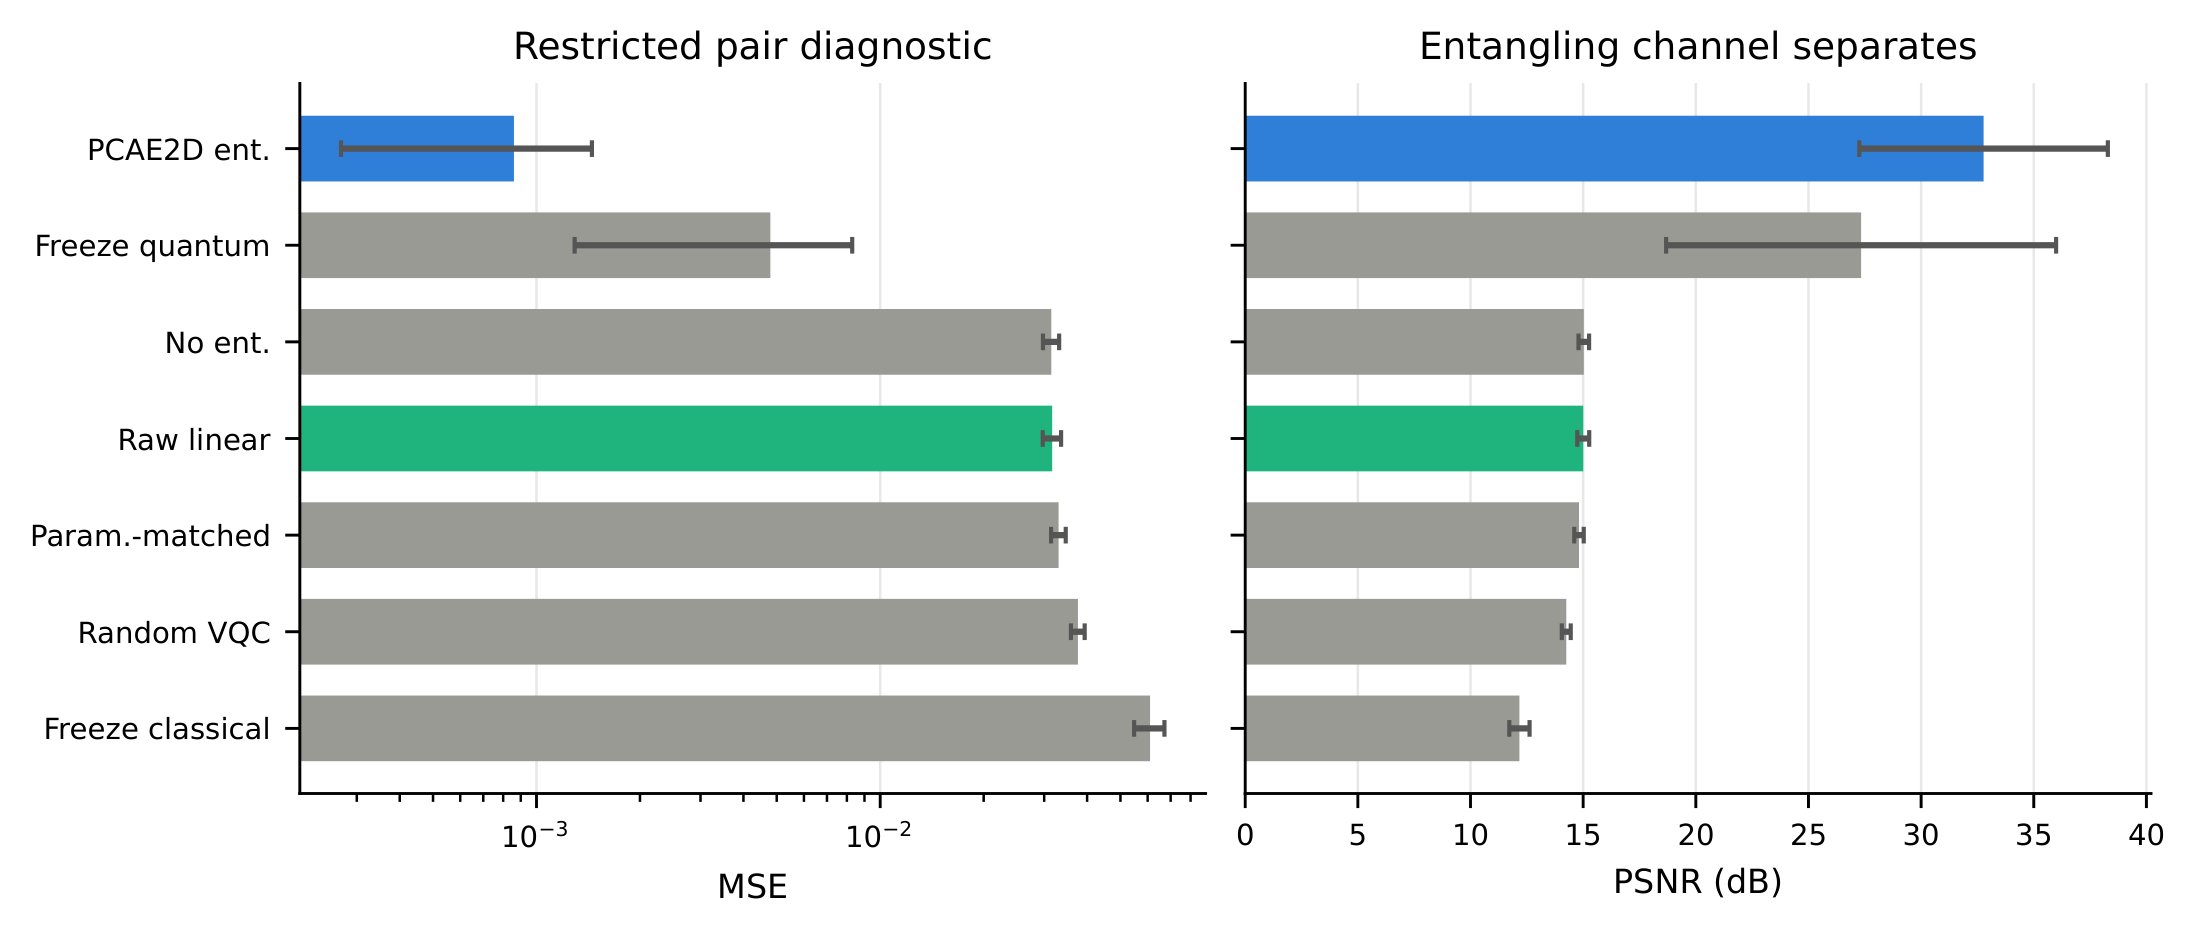
\includegraphics[width=\linewidth]{supplementary_figures/full_ablation_metric_comparison.png}
\caption{The restricted pair-correlation diagnostic underlying the entanglement-necessity result (mean $R^2=0.9735$ vs.\ $R^2\leq0.02$ for non-entangling controls), shown here as MSE (left) and PSNR (right) across the full variant set: the trained \blue{PCAE2D} entangling map, freeze-quantum, no-entanglement, raw-linear, parameter-matched classical, random-VQC, and freeze-classical. The entangling channel (blue) separates numerically from every non-entangling control on this target, in direct contrast to the ordinary held-out reconstruction result of Section~\ref{sec:holdout_headline} where the same entangling channel does not separate from local/raw controls --- the two figures together visualize this document's central task-dependence argument.}
\label{fig:restricted_diagnostic_summary}
\end{figure}

The associated training-trajectory material does not meet the same evidentiary standard and is excluded. The per-variant curves previously produced by \path{run_newhvk_suite.py::epoch_tables} are analytic interpolations from final metrics, not logged epoch measurements. Separately, the 13 stored real-image traces were recorded from \blue{PCAE2D} in training mode, whose forward pass adds Gaussian noise with standard deviation $0.01$ to every observable; their maximum one-step changes therefore mix optimizer dynamics with injected jitter. Neither source supports a training-reorganization comparison. The corrected multi-dataset runner records a noise-free evaluation-mode forward pass after each optimizer update and preserves aggregate summaries across partial runs; it was rerun across all six datasets, and Section~\ref{sec:phase_transition} reports what those corrected traces do and do not support.

\subsection{Training-Dynamics Readouts, and Why They Are Not a Transition}
\label{sec:phase_transition}
We tracked two scalar summaries of the learned representation across optimization. Neither exhibits a sharp transition: both drift smoothly, with run-to-run fluctuation. We report them here as interpretability readouts on the learned energy and entanglement, and the negative control below is why we make no stronger claim.

An earlier version of this material was withdrawn after the provenance audit above: the restricted-diagnostic trajectories previously shown were analytic interpolations produced for visualization rather than measurements from saved checkpoints, and the original multi-dataset traces were recorded during training, where \blue{PCAE2D's} training-mode forward pass deliberately adds Gaussian observable noise that confounds parameter evolution with injected jitter. The corrected runner evaluates a separate, noise-free forward pass in evaluation mode immediately after every optimizer update. It tracks the global magnetization summary $M_z(t)$, the mean of the $N$ local-$Z$ observables over all $P$ patches at optimizer step (epoch) $t$. We deliberately avoid the term ``order parameter'': $M_z$ is not associated with any symmetry breaking or transition here (the analysis below shows only smooth drift), and we use it purely as an interpretable scalar summary of the learned representation,
\begin{equation}
M_z(t) = \frac{1}{P N}\sum_{p=1}^{P}\sum_{i=1}^{N}\langle Z_i\rangle_p(t),
\label{eq:order_parameter}
\end{equation}
and the signed energy-to-entanglement ratio
\begin{align}
R_{ES}(t)&=\frac{H(t)}{S},\\
H(t)&=\sum_i\Bigl[J_x^{(i)}\langle X_iX_{i+1}\rangle
+J_y^{(i)}\langle Y_iY_{i+1}\rangle \nonumber\\
&\hspace{3.0em}+J_z^{(i)}\langle Z_iZ_{i+1}\rangle\Bigr],
\end{align}
where $S=\sum_i S_i$ is the fixed sum of von Neumann bond entropies from the classical MPS decomposition. The ratio $R_{ES}$ has units of energy per entropy unit and is \emph{not} a thermodynamic temperature: no Gibbs state is fitted, no derivative $\partial S/\partial E$ is evaluated, and its negative sign reflects the learned signed Hamiltonian. Because the MPS bond entropies are computed once from the classical decomposition and do not change during VQC training, $S$ is constant in $t$; the trace $R_{ES}(t)$ therefore tracks the learned energy $H(t)$ up to a fixed scale, and we report the ratio only to fix an interpretable energy-per-entropy scale rather than to introduce any additional dynamics. The bond correspondence is clean only for \blue{PCAE1D} at six sites, so we track it there, on two CIFAR-10 images over four seeds.

\paragraph{A within-run threshold, and the control that disqualifies it.} To test whether these traces contain anything sharper than drift, we applied a purely descriptive rule to the change magnitude $\mathcal{X}(t)=|M_z(t)-M_z(t-\Delta t)|$: flag a run when $\max_t \mathcal{X}(t)$ exceeds $\operatorname{median}_t(\mathcal{X}) + 2\operatorname{std}_t(\mathcal{X})$. That threshold is computed per run from the very trace it evaluates; it is not a fixed global constant or a null-calibrated statistical test, it supplies no $p$-value, and it controls no false-positive rate. Table~\ref{tab:phase_transition_corrected} reports what it flags across all six datasets (two images $\times$ two seeds each, 24 runs): $16/24$, a mixed and non-universal rate. Table~\ref{tab:phase_transition_onoff} is the control that settles the reading: the identical protocol applied to a \emph{classical-replacement} variant, in which the VQC is replaced by a fixed classical map and the Hamiltonian energy is identically zero throughout training, alongside matched Hamiltonian-on runs (\textit{Monalisa} and CIFAR-10 \textit{cat}, two seeds each, full 200-epoch budget). All four Hamiltonian-on runs are flagged, and so are all four Hamiltonian-off runs. The rule cannot distinguish a Hamiltonian-driven change from one it would flag in a change-magnitude trace regardless of whether any physical energy term is present in the model at all. We therefore report no transition, no critical epoch, and no critical temperature anywhere in this work; what survives is the trace itself, read as a diagnostic.

\begin{table}[H]
\centering
\caption{Within-run threshold rule applied to the corrected, noise-free $M_z(t)$ traces across all six datasets (2 images $\times$ 2 seeds/dataset). ``Flagged'' counts runs whose sharpest change exceeds that run's own threshold; it is a descriptive tally, not a detection claim, and the control in Table~\ref{tab:phase_transition_onoff} shows it is not sensitive to the Hamiltonian term.}
\label{tab:phase_transition_corrected}
\scriptsize
\begin{tabular}{lcccc}
\toprule
Dataset & $n$ & Flagged & Mean flagged epoch & Mean $\mathcal{X}_{\max}$ \\
\midrule
CIFAR-10 & 4 & 2/4 & 64.0 & $0.0036\pm0.0009$ \\
MNIST & 4 & 4/4 & 98.75 & $0.0023\pm0.0012$ \\
Fashion-MNIST & 4 & 2/4 & 45.0 & $0.0027\pm0.0011$ \\
PathMNIST & 4 & 2/4 & 54.5 & $0.0038\pm0.0015$ \\
BloodMNIST & 4 & 3/4 & 96.0 & $0.0033\pm0.0012$ \\
PneumoniaMNIST & 4 & 3/4 & 103.0 & $0.0036\pm0.0008$ \\
\midrule
Total & 24 & $16/24$ & -- & -- \\
\bottomrule
\end{tabular}
\end{table}

\begin{table}[H]
\centering
\caption{The negative control (200 epochs, two seeds/image). ``On'' is the standard Hamiltonian-regularized model; ``off'' is the classical-replacement variant with energy identically zero throughout training. The threshold rule fires in every case tested, in both conditions --- which is why no transition is claimed.}
\label{tab:phase_transition_onoff}
\scriptsize
\begin{tabular}{llccc}
\toprule
Image & Seed & Hamiltonian & Flagged & Flagged epoch \\
\midrule
Monalisa & 0 & On & Yes & 4 \\
Monalisa & 0 & Off & Yes & 8 \\
Monalisa & 1 & On & Yes & 162 \\
Monalisa & 1 & Off & Yes & 23 \\
CIFAR cat & 0 & On & Yes & 97 \\
CIFAR cat & 0 & Off & Yes & 6 \\
CIFAR cat & 1 & On & Yes & 105 \\
CIFAR cat & 1 & Off & Yes & 1 \\
\midrule
Total & \multicolumn{2}{c}{On} & 4/4 & -- \\
Total & \multicolumn{2}{c}{Off} & 4/4 & -- \\
\bottomrule
\end{tabular}
\end{table}

\begin{figure}[H]
\centering
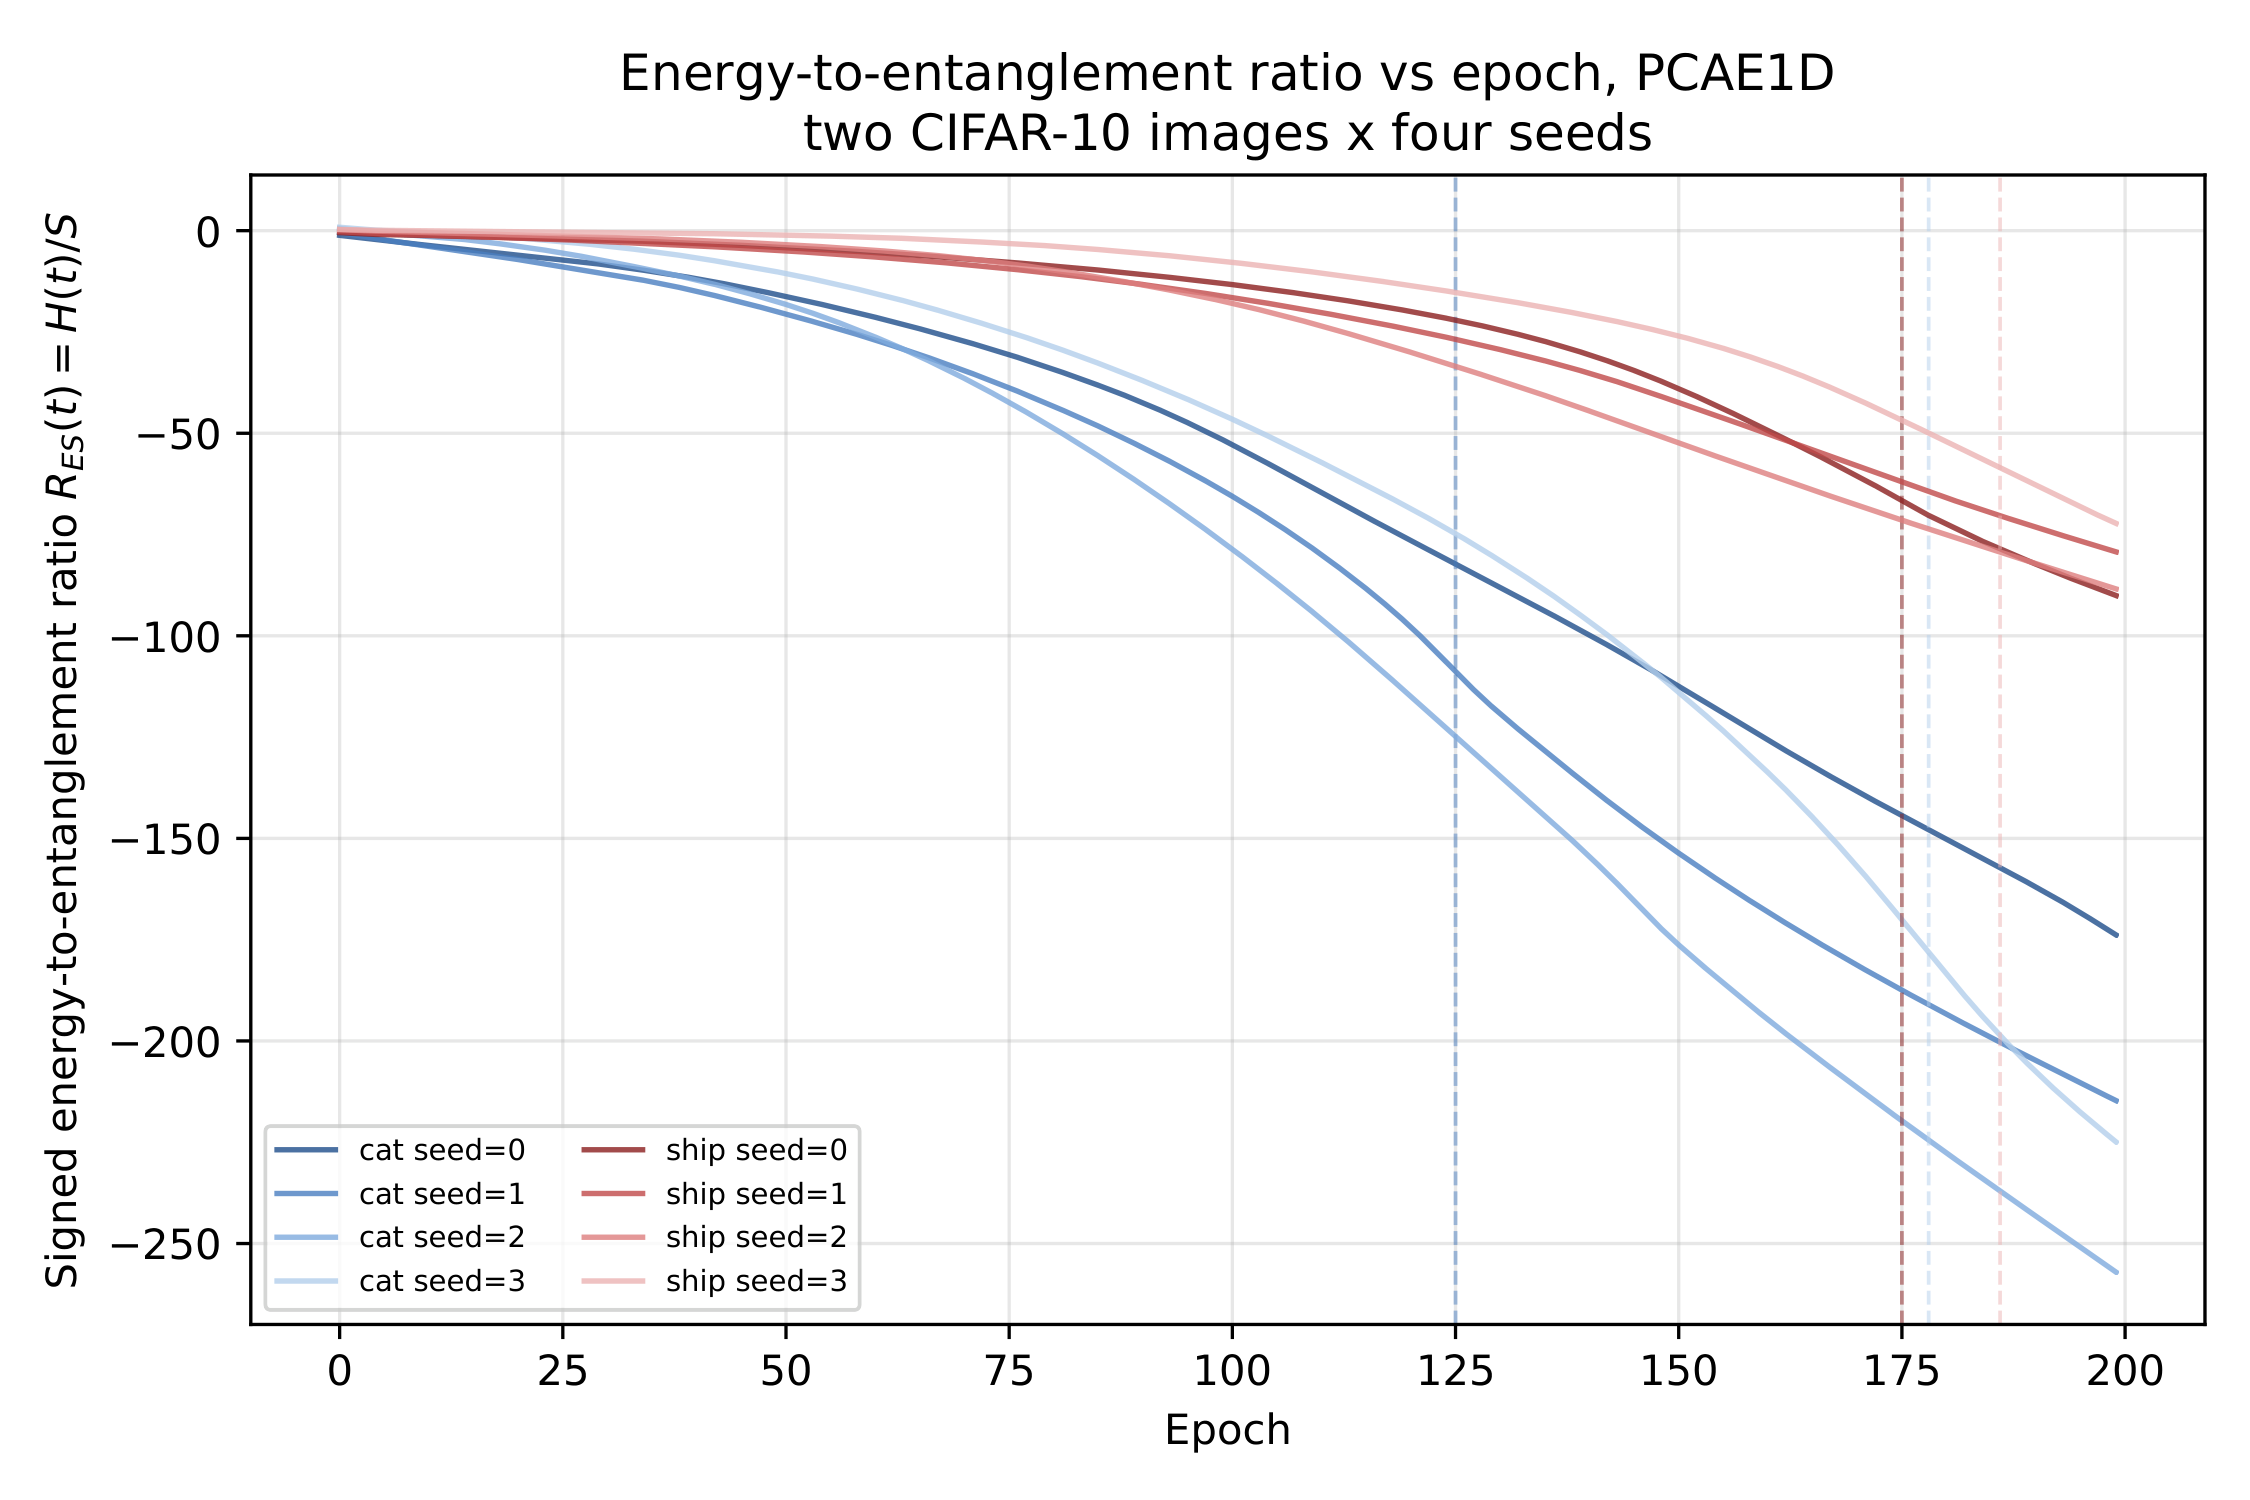
\includegraphics[width=\linewidth]{supplementary_figures/critical_temperature_traces.png}
\caption{The surviving readout: signed energy-to-entanglement ratio $R_{ES}(t)=H(t)/S$ across training, \blue{PCAE1D,} two CIFAR-10 images $\times$ four seeds. Every trace descends smoothly and monotonically as the learned signed energy decreases at fixed $S$. There is no sharp feature here, and none is claimed: these are not temperature or cooling curves, and no critical epoch is marked. The figure is shown because this smooth descent is what the Hamiltonian term makes legible --- an interpretability readout a purely classical feature map does not natively expose.}
\label{fig:critical_temperature}
\end{figure}

All eight $R_{ES}$ traces behave this way (Figure~\ref{fig:critical_temperature}). The smooth, monotone descent --- not any threshold crossing --- is the interpretable content, and it is the sense in which we claim an ``interpretable Hamiltonian diagnostic'' as a capability.


\section{\blue{PCAE1D} versus \blue{PCAE2D:} A Direct Topology Comparison}
\label{sec:topology_comparison}
The main paper introduces both the \blue{PCAE1D} (6-qubit chain) and \blue{PCAE2D} ($2\times3$ grid) topologies, but until now the only direct comparison was the same-set CIFAR-10 fit reported above. Here we compare the two topologies directly under matched conditions --- identical qubit count (6, native to both), identical feature width, identical decoder architecture and step budget --- on held-out generalization rather than same-set fitting, on two evidence bases: a fast analytic-surrogate sweep at full statistical scope, and a smaller real-trained-circuit confirmation subset. The two topologies are close in parameter count by construction \blue{(PCAE1D:} 53{,}787; \blue{PCAE2D:} 52{,}755) but not identical, since their circuit structures differ (chain vs. grid connectivity, 27 vs. 19 measured observables); we report this honestly rather than forcing an artificial match.

\subsection{Real-Circuit Confirmation}
\label{sec:topology_real_circuit}
Each topology was trained jointly on 2 CIFAR-10 images (native $32\times32$, overlapping $8\times8$ patches at stride 4, 49 patches/image --- the same convention as the same-set CIFAR-10 protocol above) for a reduced 90-step budget across 3 seeds, then evaluated by direct forward pass (no retraining) on 3 further CIFAR-10 images from different classes never seen in training (airplane, frog, automobile) --- a genuine held-out test. The reduced step budget and seed count follow directly from a measured \blue{Thermodynamictiming} calibration on this project's GPU (NVIDIA GTX 1050): at the full 200-step budget used elsewhere in this document, the complete topology comparison at the scope below would cost single-digit hours rather than the tens of minutes actually spent; we report this budget explicitly rather than silently shrinking scope.

\begin{table}[H]
\centering
\caption{Real-trained-circuit topology comparison: held-out reconstruction on 3 unseen CIFAR-10 images (9 image-seed pairs per topology: 3 seeds $\times$ 3 held-out images), 90-step budget.}
\label{tab:topology_real_circuit}
\scriptsize
\begin{tabular}{lcccc}
\toprule
Topology & Params & Held-out PSNR (dB) & Held-out SSIM & Wall time / run (min) \\
\midrule
\blue{PCAE1D} & 53{,}787 & $11.73\pm1.99$ & $0.317\pm0.227$ & $29.6\pm9.0$ \\
\blue{PCAE2D} & 52{,}755 & $11.57\pm1.53$ & $0.304\pm0.188$ & $16.6\pm0.3$ \\
\bottomrule
\end{tabular}
\end{table}

The two topologies \blue{have similar} held-out \blue{PSNR} means at this scale. Across the 9 image--seed pairs, the paired \blue{PCAE1D-minus-PCAE2D} difference is $0.16$~dB. After aggregating the three image differences within each seed, the seed-bootstrap 95\% CI is $[-0.38,0.46]$~dB and the two-sided Wilcoxon test gives $p=0.50$. The 3-seed, 3-image subset is too small to establish formal equivalence. \blue{PCAE2D} nevertheless completes the same 90-step budget in roughly half the wall-clock time of \blue{PCAE1D} at a comparable parameter count, a measured resource-cost difference. This is consistent with \blue{PCAE2D's} smaller measured observable set (19 vs.\ 27); the corresponding transpiled depth and two-qubit-gate counts are shown in Figure~\ref{fig:ibm_circuit_summary}. At the tested scale, the evidence supports treating topology primarily as a resource-cost choice rather than claiming an accuracy difference.

\paragraph{\blue{Random-latent floor.}} The $\sim\!11.7$~dB above is close to the random-latent range quoted elsewhere in this study, so we measured the floor directly rather than leaving the question open: a random-VQC control under the identical protocol --- same two training images, same overlapping $8\times8$ patches at stride 4, same 90 steps, same learning rate per topology, same three held-out images and seeds, with the observable vector replaced by resampled noise and the decoder trained normally --- reaches $12.74\pm2.21$~dB \blue{(PCAE1D)} and $12.64\pm2.12$~dB \blue{(PCAE2D).} The trained circuits are therefore \emph{below} their own floor by about $1$~dB ($-1.01$ and $-1.08$~dB on the means), and the paired difference is negative in all six seed-level comparisons (two-sided Wilcoxon $p=0.031$ over the six seed means). At 90 steps neither model has trained far enough for its latent to beat an input-independent predictor, which is what a decoder fed pure noise converges to. The absolute numbers in Table~\ref{tab:topology_real_circuit} must accordingly not be read as reconstruction quality; only the \blue{PCAE1D-minus-PCAE2D} \emph{difference} is meaningful here, and even that is a comparison between two runs measured before either clears the floor. The full-scope surrogate sweep of Section~\ref{sec:topology_surrogate}, not this subset, is what supports the topology conclusion. Control driver: \path{Main2/newHVK/run_topology_random_vqc_control.py}; artifact \path{Main2/newHVK/results/topology_comparison/random_vqc_control.json}.

\subsection{Surrogate Sweep: Full Statistical Scope}
\label{sec:topology_surrogate}
To reach the seed and dataset breadth a held-out comparison needs, we extend the analytic-surrogate held-out framework used above (Tables~\ref{tab:hvk_real_cifar} and~\ref{tab:multi_dataset_reconstruction}) with an \blue{PCAE1D-equivalent} feature map. The \blue{PCAE2D} surrogate used there (\texttt{real\_newhvk\_features}) is a closed-form proxy built from six index-pairs of the local-observable block, standing in for the grid circuit's pairwise $ZZ$ correlators. The new \blue{PCAE1D} surrogate is not a relabeled copy: it iterates the chain topology's actual five nearest-neighbor bonds (vs.\ the grid's seven-edge pattern) and adds a second, distinct pair-type term reflecting \blue{PCAE1D's} extra $XX$/$YY$ measurement channels that the 2D grid circuit does not have (it measures only $Z$, $X$, $ZZ$). Both surrogates share the same local/positional input convention, so the comparison is apples-to-apples. We run the full held-out reconstruction and downstream-classification battery (5 seeds, stratified splits) across CIFAR-10, Fashion-MNIST, and PathMNIST.

\begin{figure*}[t]
\centering
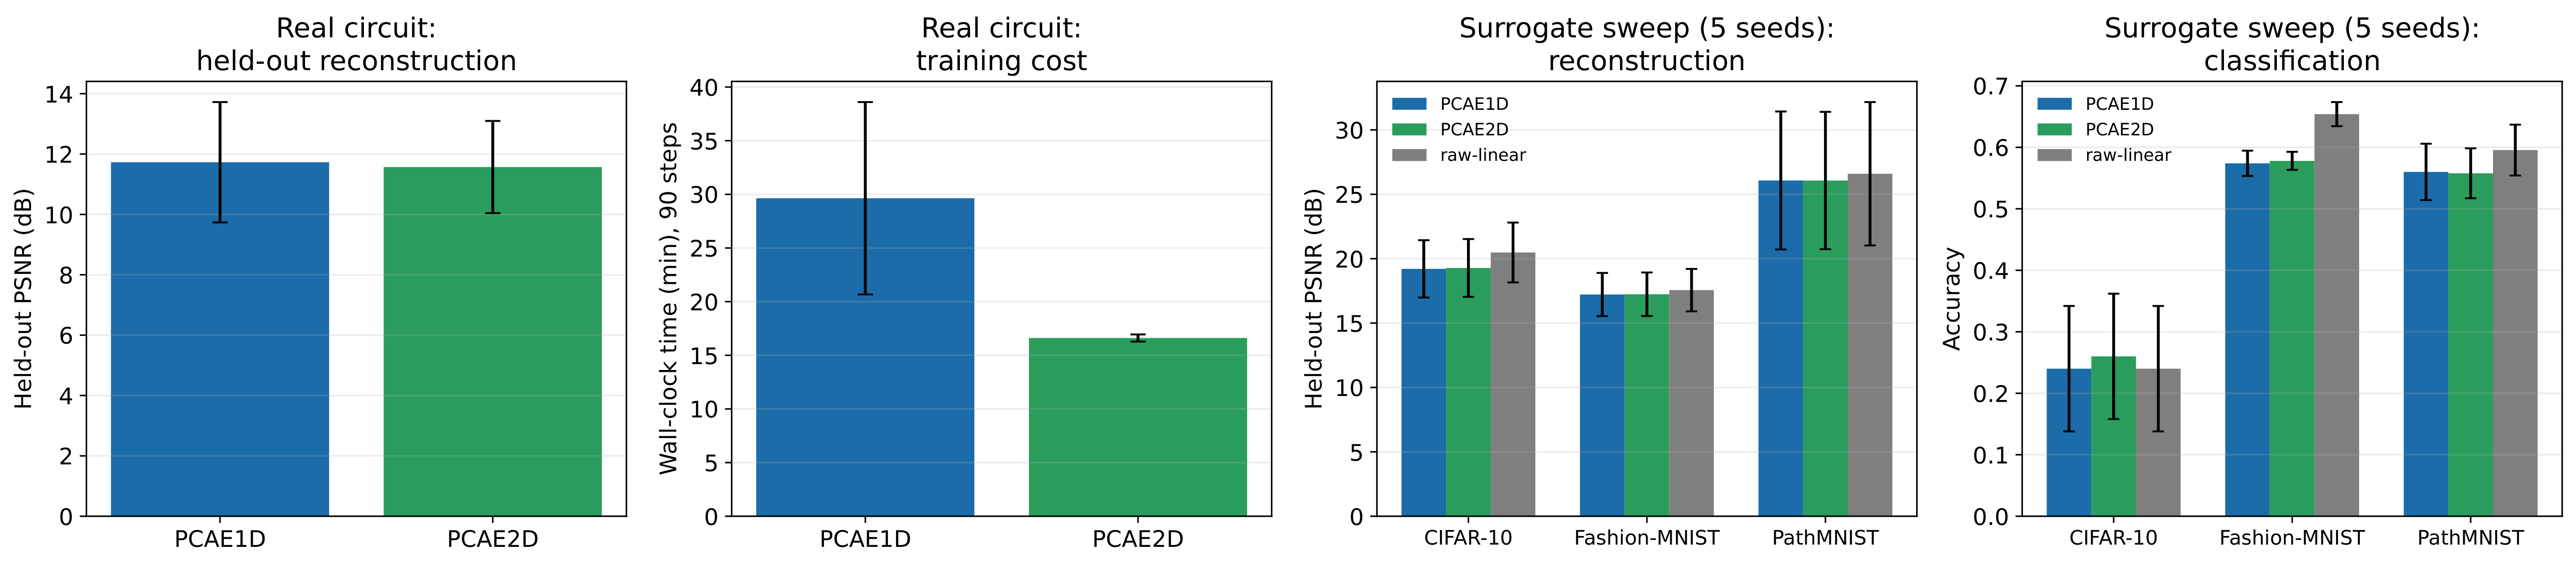
\includegraphics[width=0.95\textwidth]{supplementary_figures/topology_comparison_summary.png}
\caption{\blue{PCAE1D} vs.\ \blue{PCAE2D} across both evidence bases. Left two panels: real-circuit held-out PSNR and per-run wall-clock time (90-step budget, 3 seeds, error bars = std). Right two panels: surrogate-sweep held-out reconstruction PSNR and classification accuracy across three datasets (5 seeds), both topologies plotted against the strongest classical control (raw-linear).}
\label{fig:topology_comparison_summary}
\end{figure*}

The broader surrogate sweep reproduces the real-circuit pattern: \blue{PCAE1D-pair} and \blue{PCAE2D-pair} track each other closely on every dataset and metric (PSNR differs by at most $0.07$~dB, accuracy by at most $2$ percentage points), and both sit slightly below the raw-linear control. For inference, held-out image differences are first averaged within each split seed so that images sharing a fitted readout are not treated as independent replicates. The seed-level \blue{PCAE1D-minus-PCAE2D} PSNR differences are $-0.070$~dB on CIFAR-10 (bootstrap 95\% CI $[-0.151,0.024]$, Wilcoxon $p=0.3125$), $-0.021$~dB on Fashion-MNIST (CI $[-0.033,-0.006]$, $p=0.125$), and $0.003$~dB on PathMNIST (CI $[-0.012,0.015]$, $p=0.625$), all at $n=5$ seeds. The Fashion-MNIST percentile interval excludes zero, but the discrete seed-level signed-rank test does not resolve the difference; we therefore describe it as numerically small rather than statistically established. Neither topology shows a general reconstruction/classification advantage over simple classical baselines, and the evidence supports treating topology as a resource-cost choice at the tested scale. Section~\ref{sec:restricted_ablation}'s restricted, leakage-audited diagnostic remains the setting where entanglement structure matters within the tested feature/readout class.


\section{\blue{$D_4$ Pooling on the Trained Circuit}}
\label{sec:d4_real_circuit}
\blue{The main paper checks $D_4$ pooling on the closed-form surrogate map. Two quantities}
\blue{are used here. The feature-equivariance error compares the observable grid of a}
\blue{transformed image with the correspondingly permuted grid of the original image. The}
\blue{output consistency is found by reconstructing an image from each of its eight}
\blue{$D_4$-transformed copies, transforming each reconstruction back to the original}
\blue{orientation, and taking the mean squared disagreement between the eight results.}
This section \blue{checks} pooled-vs-non-pooled equivariance and \blue{output consistency} on the \emph{actual trained quantum circuit}, using the same four already-trained \blue{PCAE2D} checkpoints used for the main paper's real IBM-hardware pilot (\textit{cat}, \textit{ship/hydrofoil}, \textit{ship/sea boat}, \textit{airplane}), replayed with no retraining. For each image we run the trained model's real PennyLane forward pass (exact statevector simulation of the trained weights, not the surrogate formula) on all eight $D_4$-transformed copies of the full image, and compute both quantities, both without pooling and with the identical Reynolds-averaging construction applied to the real circuit's own output grid.

Across all four checkpoints the result is unambiguous. Without pooling, the mean feature-equivariance error is $0.2777$ and the mean output-consistency MSE is $4.355\times10^{-2}$; with the identical Reynolds-averaging construction applied to the real circuit's own output grid, these fall to $5.39\times10^{-8}$ and $1.46\times10^{-15}$ respectively --- the latter at the numerical floor of double precision. Per-image values for all four checkpoints are in the machine-readable archive. The equivariance is therefore exact by construction on the trained circuit, not only on the analytic surrogate.

The real-circuit result confirms the surrogate's finding directly: pooling collapses the equivariance error from $\mathcal{O}(10^{-1})$ to $\mathcal{O}(10^{-8})$ and output-consistency MSE from $\mathcal{O}(10^{-2})$ to $\mathcal{O}(10^{-15})$, an 8--13 order-of-magnitude gap on every one of the four images, with no exceptions. The pooled real circuit's residual error ($\sim\!5\times10^{-8}$) is larger than the surrogate's floating-point-precision result ($\sim\!10^{-17}$) because the real circuit involves a full statevector simulation of the trained gates plus a fresh per-transform feature-standardization step, both of which accumulate ordinary floating-point noise that the closed-form surrogate formula does not --- the pooled result is exact up to numerical precision, not exact to the same sixteen digits as a symbolic identity, which is the expected and unremarkable difference between an analytic proxy and an actual simulated circuit.


\section{Exact Circuit and Hamiltonian Definitions}
\label{sec:supp_exact_circuits}
For a one-dimensional chain of $n_{\text{bonds}}$ bonds indexed by $i$ and sites $(i,i+1)$, the anisotropic Heisenberg Hamiltonian is
\begin{align}
H_{\text{Heis}}=\sum_{i=0}^{n_{\text{bonds}}-1}\Bigl(
J_x^{(i)}X_iX_{i+1}+J_y^{(i)}Y_iY_{i+1}\nonumber\\
{}+J_z^{(i)}Z_iZ_{i+1}\Bigr).
\end{align}
Here $X,Y,Z$ are Pauli operators and $J_\alpha^{(i)}$ are bond-resolved couplings. \blue{PCAE1D} fixes six sites and treats the 15 coefficients on its five bonds as learnable parameters initialized independently from a zero-mean Gaussian with standard deviation $0.1$. Given patch $n$'s measured observables, its energy diagnostic is
\begin{equation}
\mathcal{E}_n(\theta,J) = \sum_{i=0}^{4}\sum_{\alpha\in\{x,y,z\}} J_\alpha^{(i)}\langle\sigma_\alpha^{(i)}\sigma_\alpha^{(i+1)}\rangle_n.
\end{equation}
\blue{PCAE2D} instead uses the seven edges $\mathcal{G}_{2D}$ of its $2\times3$ circuit graph and the implemented grid-Ising diagnostic $\mathcal{E}^{2D}_n=\sum_{(u,v)\in\mathcal{G}_{2D}}j_{uv}\langle Z_uZ_v\rangle_n$. Thus ``Hamiltonian diagnostic'' refers to the full $XX/YY/ZZ$ chain energy for \blue{PCAE1D} and the learned $ZZ$ graph energy for \blue{PCAE2D.} In either case, the patch-averaged term is $\mathcal{L}_{\text{energy}}=\frac{1}{N}\sum_n \mathcal{E}_n$, and the total objective is
\begin{align}
\mathcal{L}_{\text{total}}&=\mathcal{L}_{\text{rec}}
+\lambda\,\mathcal{L}_{\text{energy}},\\
\mathcal{L}_{\text{rec}}&=\frac{1}{N}\sum_{n=1}^{N}
\bigl\|D(o_n,e_n)-P_n\bigr\|_F^2.
\end{align}
with $D$ the classical decoder and $P_n$ the ground-truth patch.

\begin{sloppypar}
Per-patch coordinates $(r_i,c_j)$ are mapped to Fourier features $e_{4k}=\sin(\omega_k\pi r_i)$, $e_{4k+1}=\cos(\omega_k\pi r_i)$, $e_{4k+2}=\sin(\omega_k\pi c_j)$, and $e_{4k+3}=\cos(\omega_k\pi c_j)$ \cite{Xu2021}. \blue{PCAE1D} uses $k\in\{0,1\}$ (8-D), whereas the native-resolution \blue{PCAE2D} implementation uses one frequency (4-D); a learned linear map projects either vector to six $R_Y$ angles. Both six-qubit circuits first apply $U_{\text{enc}}(x_n)=\bigotimes_{i=0}^{5}R_X(x_n^{(i)})$ and $U_{\text{pos}}=\bigotimes_{i=0}^{5}R_Y(\theta_{\text{position}}^{(i)})$. Each of two \blue{PCAE1D} layers then applies per-qubit $\mathrm{Rot}$ gates followed by the strongly-entangling CNOT ring. Each \blue{PCAE2D} layer applies CNOTs over the four horizontal and three vertical grid edges followed by per-qubit $\mathrm{Rot}$ gates, matching the executed source and hardware-replay circuits.

\blue{PCAE1D} returns local $Z/X$ measurements and the three nearest-neighbor pair sectors $ZZ/XX/YY$ (27 values); \blue{PCAE2D} returns local $Z/X$ measurements and grid-edge $ZZ$ correlations (19 values). Positional rotations and fixed graph connectivity distinguish circuit sites, so neither unpooled map is asserted to be permutation- or $D_4$-equivariant. The $D_4$ action in the main paper is instead the explicit permutation action on the $4\times4$ patch grid, and equivariance follows only after the stated Reynolds average over its eight transformations.
\end{sloppypar}

\section{Hardware Pilot Methodology}
\label{sec:hardware_methodology}
The main paper reports a real IBM Quantum hardware reconstruction pilot (five images: \textit{Monalisa} and four CIFAR-10 images, each optimized per-image, hardware PSNR $25.90$--$31.52$~dB against $36.56$--$46.79$~dB in noiseless simulation). This section gives the complete methodology.

\subsection{Reused Checkpoints}
No model was retrained for this pilot. Two pre-existing artifacts were reused directly. The first was the ``shared VQC baseline'' Monalisa checkpoint under
\begin{quote}
\small\path{main2/newHVK/results/ablation_study/legacy_hvk_controls/eval_controls/}\newline\path{shared-baseline-seed-42/}.
\end{quote}
This is the run underlying the \blue{``Legacy baseline, signed energy'' row of the Hamiltonian-sector controls table in the main paper}. The second set comprised four fresh \blue{PCAE2D} checkpoints trained for 200 steps with Adam ($\eta=0.004$) on an NVIDIA GTX~1050. Each checkpoint corresponds to one native-resolution $32\times32$ CIFAR-10 image optimized directly on its own target, following the same per-image protocol as \textit{Monalisa} rather than the held-out suite of Section~\ref{sec:holdout_headline}. Non-overlapping $8\times8$ patches give 16 patches per image, matching the Monalisa pilot's patch count and keeping the hardware circuit budget predictable.

\subsection{Circuit Reconstruction}
The trained \blue{PCAE1D} forward pass applies, per patch: $R_X$ angle embedding, $R_Y$ positional modulation, then two \texttt{StronglyEntanglingLayers} (per-wire $R_Z$-$R_Y$-$R_Z$ rotations with a CNOT ring whose range increments by layer). We rebuilt this gate-for-gate in Qiskit. Because the trained circuit measures $Z$, $X$, $ZZ$, $XX$, and $YY$ (27 observables), and pairwise correlators are recoverable as joint parities of the \emph{same} all-$Z$/all-$X$/all-$Y$ basis measurements that already give the single-qubit marginals, only three measurement circuits per patch are needed. For 16 Monalisa patches this is $16\times3=48$ circuits. The \blue{PCAE2D} grid circuit is simpler (two layers of fixed grid-edge CNOTs then per-qubit rotations) and measures only $Z$, $X$, $ZZ$ (19 observables, no $XX$/$YY$), so only two measurement circuits per patch are needed: for four CIFAR images at 16 patches each, $4\times16\times2=128$ circuits.

\begin{figure}[H]
\centering
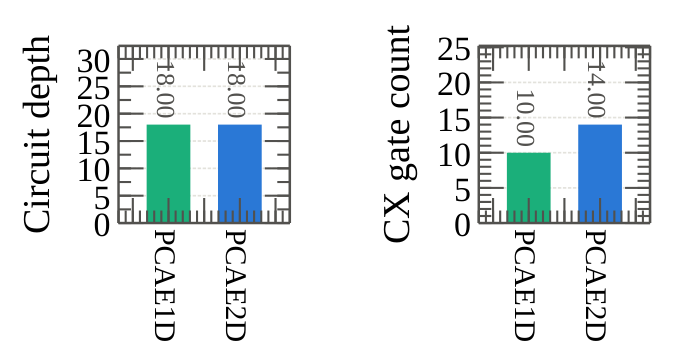
\includegraphics[width=0.75\linewidth]{supplementary_figures/ibm_circuit_summary.png}
\caption{Transpiled circuit resource comparison between the \blue{PCAE1D} (\textit{Monalisa}) and \blue{PCAE2D} (CIFAR) per-patch circuits at \texttt{optimization\_level=1} on \texttt{ibm\_fez}: circuit depth (left) and CX-gate count (right). Both circuits have depth 18 and use 10--14 CX gates. These resource counts document the executed circuits; they do not by themselves attribute the observed hardware--simulator PSNR gap to a particular noise source.}
\label{fig:ibm_circuit_summary}
\end{figure}

\subsection{Local Validation Before Any Hardware Submission}
Every circuit was validated against the cached, training-time observable vectors via an exact Qiskit statevector simulation, \emph{before} any job was submitted to real hardware. Sixteen patches were validated per checkpoint across all five checkpoints; the maximum absolute reconstruction error was $7.89\times10^{-4}$ for Monalisa \blue{(PCAE1D)} and $7.14\times10^{-6}$--$9.42\times10^{-6}$ for the four CIFAR \blue{PCAE2D} checkpoints.

All translation discrepancies are small relative to the observable perturbations induced by finite-shot device execution: across the five checkpoints, the hardware--statevector mean absolute observable deviation is $0.096$--$0.125$ (maximum $0.218$--$0.340$), versus a maximum translation discrepancy of $7.89\times10^{-4}$ for Monalisa and $9.42\times10^{-6}$ for CIFAR. They therefore rule out a gate-translation mismatch of the measured magnitude as the primary explanation for the hardware--simulator PSNR gap. This pilot does not separate sampling noise, gate/readout errors, drift, and transpilation effects.

\subsection{Reconstruction Decode}
Hardware counts were converted to observable expectation values by the standard parity estimator, $\langle Z_i\rangle = \frac{1}{S}\sum_{\text{shots}} (-1)^{b_i}$ (identically for $X$, $Y$ after basis rotation), with pairwise correlators computed as the shot-weighted mean of $(-1)^{b_i+b_j}$ within the same measurement basis. The resulting observable vector, concatenated with the training-time positional encoding, was passed through the \emph{unmodified} trained decoder. No hardware-specific fine-tuning, error mitigation, or post-hoc calibration was applied.


\section{\blue{Reproducibility and Training Settings}}
\label{sec:training_settings}
The repository-level experiment drivers set Python, NumPy, and PyTorch random seeds explicitly. Unless a section states otherwise, multi-seed studies use seeds $\{0,1,2,3,4\}$; the reduced real-circuit topology confirmation and six-dataset reconstruction extension use $\{0,1,2\}$. Held-out samples are disjoint from their corresponding fitting samples, and each reported paired test preserves the pairing unit stated in its table or surrounding text (image within split, or seed after within-seed image aggregation). ``Mean $\pm$ std'' denotes the arithmetic mean and population-standard-deviation summary (NumPy \texttt{ddof=0}) over the unit named in the caption. Bootstrap intervals are percentile 95\% intervals; Wilcoxon values are two-sided signed-rank tests. No multiple-comparison correction is applied, so $p$-values should be interpreted as individual-comparison summaries rather than as a family-wise discovery analysis. {\color{red}\textbf{[Student: this sentence says no multiple-comparison correction is applied, but the
TOST verdicts of Section~\ref{sec:holdout_headline} now use Holm correction. Please reword it so the two agree.]}}

The current verification environment uses Python 3.11.9, PyTorch 2.6.0 with CUDA 12.4, PennyLane 0.42.3, Qiskit 2.5.0, NumPy 2.4.6, pandas 3.0.3, scikit-learn 1.9.0, quimb 1.11.2, cotengra 0.7.5, and autoray 0.6.12 on an NVIDIA GeForce GTX 1050. The package constraints are declared in \path{pyproject.toml}; because that file does not pin every dependency to an exact version, the versions above identify the environment used for this verification pass rather than claiming bitwise reproducibility across arbitrary future installations.

\blue{Table~\ref{tab:training_settings} lists the training settings of each experiment. All}
\blue{trained models use Adam with full-batch updates over the patches of their training}
\blue{images. The loss is the reconstruction mean squared error plus $\lambda=0.01$ times the}
\blue{mean Hamiltonian energy, except where an ablation removes or replaces the energy term.}
\blue{The held-out comparison fits no network. Its linear readout is solved in closed form as a}
\blue{ridge regression with regularisation $10^{-6}$.}

\begin{table}[H]
\centering\color{blue}
\caption{Training settings. Learning rates are for Adam. Patches are non-overlapping unless a stride is given.}
\label{tab:training_settings}
\footnotesize
\setlength{\tabcolsep}{4pt}
\begin{tabular}{@{}l l l r l l@{}}
\toprule
Experiment & Model & Patches & Steps & Learning rate & Seeds \\
\midrule
\textit{Monalisa} fit$^{a}$ & PCAE1D & 16, $64\times64$ & 200 & 0.003 & 42 \\
240-step ablation & PCAE1D & 16, $64\times64$ & 240 & 0.003 & 0, 1, 2 \\
Six-dataset fits & PCAE2D & 16, $8\times8$ & 80--100 & 0.004 & -- \\
CIFAR-10 hardware fits & PCAE2D & 16, $8\times8$ & 200 & 0.004 & -- \\
Topology comparison & 1D / 2D & 49, $8\times8$, stride 4 & 90 & 0.003 / 0.004 & 0, 1, 2 \\
Held-out comparison & surrogate & 16, $8\times8$ & -- & closed form & 0--4 \\
\bottomrule
\end{tabular}

\smallskip
\raggedright $^{a}$\,Used for the hardware pilot and the Hamiltonian-term controls.
\end{table}
{\color{red}\textbf{[Student: the values in Table~\ref{tab:training_settings} are read from the
training scripts and their default settings (\path{Main/src/training/training.py},
\path{run_full_dataset_sameset.py}, \path{train_and_save_hvk2d_checkpoints.py},
\path{run_topology_comparison.py}, \path{run_core_multiseed_240.py},
\path{run_newhvk_suite.py}). Please confirm that the reported runs used them, fill in the
seeds marked ``--'', and check the patch layout of the held-out comparison.]}}


\section*{\blue{Relationship to the main manuscript}}
\blue{The main paper reports per-image reconstruction, the five-image IBM hardware pilot,}
\blue{feature-level $D_4$ pooling, the restricted pair-observable diagnostic, and the}
\blue{Holm-corrected held-out equivalence verdict. This supplement gives the per-seed and}
\blue{per-control results behind them, the negative controls, the topology comparison, the}
\blue{$D_4$ check on the trained circuit, the hardware methodology, the training settings,}
\blue{and the provenance audits. The held-out comparison uses a closed-form 32-D surrogate of}
\blue{the PCAE2D observable map. It should not be confused with the 19-D PCAE2D circuit used}
\blue{for per-image reconstruction. The $D_4$ group average is a feature-grid diagnostic, not}
\blue{an end-to-end trained reconstruction operator.}


\begin{thebibliography}{9}
\bibitem{Schuirmann1987TOST} D. J. Schuirmann, ``A comparison of the two one-sided tests procedure and the power approach for assessing the equivalence of average bioavailability,'' \textit{Journal of Pharmacokinetics and Biopharmaceutics}, vol. 15, no. 6, pp. 657--680, 1987, doi: 10.1007/BF01068419.
\bibitem{Lakens2017TOST} D. Lakens, ``Equivalence tests: A practical primer for $t$ tests, correlations, and meta-analyses,'' \textit{Social Psychological and Personality Science}, vol. 8, no. 4, pp. 355--362, 2017, doi: 10.1177/1948550617697177.
\bibitem{Krizhevsky2009} A. Krizhevsky, ``Learning multiple layers of features from tiny images,'' University of Toronto, Technical Report, 2009.
\bibitem{LeCun1998} Y. LeCun, L. Bottou, Y. Bengio, and P. Haffner, ``Gradient-based learning applied to document recognition,'' \textit{Proceedings of the IEEE}, vol. 86, no. 11, pp. 2278--2324, 1998, doi: 10.1109/5.726791.
\bibitem{Xiao2017} H. Xiao, K. Rasul, and R. Vollgraf, ``Fashion-MNIST: A novel image dataset for benchmarking machine learning algorithms,'' arXiv:1708.07747, 2017.
\bibitem{Yang2023} J. Yang et al., ``MedMNIST v2---A large-scale lightweight benchmark for 2D and 3D biomedical image classification,'' \textit{Scientific Data}, vol. 10, Art. no. 41, 2023, doi: 10.1038/s41597-022-01721-8.
\bibitem{Wolberg1993} W. Wolberg, O. Mangasarian, N. Street, and W. Street, ``Breast Cancer Wisconsin (Diagnostic),'' UCI Machine Learning Repository, 1993, doi: 10.24432/C5DW2B.
\bibitem{Xu2021} R. Xu, X. Wang, K. Chen, B. Zhou, and C. C. Loy, ``Positional Encoding as Spatial Inductive Bias in GANs,'' in \textit{Proceedings of the IEEE/CVF Conference on Computer Vision and Pattern Recognition (CVPR)}, 2021, pp. 13569--13578.
\end{thebibliography}

\end{document}
